%%%%%%%%%%%%%%%%%%%%%%%%%%%%%%%%%%%%%%%%%%%%%%%%%%%%%%%%%%%%%%%%
\chapter{感情音声の選別と尺度評定}
\label{sec:DBScreening}
%%%%%%%%%%%%%%%%%%%%%%%%%%%%%%%%%%%%%%%%%%%%%%%%%%%%%%%%%%%%%%%% 
感情音声を用いた実験では、結果がその音声の特性に大きく影響される可能性があるため、音声の選別作業を行なった。
本章では、使用した音声データベースの詳細と、本文\ref{sec:PrepareStimuli}節・\ref{sec:PrepareStimuli_cal}節で
で述べた感情音声の選別作業と感情尺度評定の手順について詳しく説明する。

%%--------------------------------------------------------------
\section{音声データベースについて}
\label{sec:Keio-ESD}
%%--------------------------------------------------------------
本研究では、慶應義塾大学研究用感情音声データベース(Keio-ESD)\cite{keioESD-J}を使用した。
本データベースには、一般人男性話者1名(32歳,舞台経験あり)が47感情で発声した20単語の音声と、
感情音声合成システムによって合成された音声が含まれる。
今回は、前者の収録された音声を使用することにした。
収録音声数は、話者1名 $\times$ 20単語 $\times$ 46感情(平静を除く) + 複数回収録の平静音声の全1025音声である。
単語と感情の詳細を図\ref{fig:Keio-ESD}に示す。
なお、本研究では図中の赤色の行に示す名詞11単語を最初に用いることとした。
名詞を用いたのは、それ以外の単語の感情発話がイメージしづらく、名詞の方がより正確に感情をのせて発話できているのではないかと考えたためである。



% ----------------------------------%
\begin{figure}[t]

  \begin{tabular}{cc}
  \begin{minipage} {0.45\hsize}
  \centering
  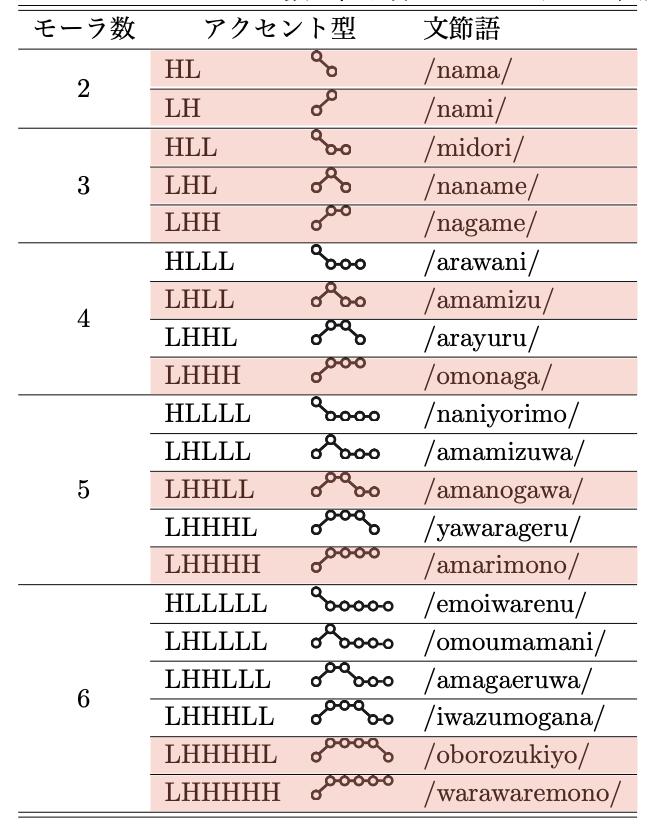
\includegraphics [ width = 1\columnwidth]{Figure/Appendix/6A/Table_Keio-ESD_Vocab.eps}
  \end{minipage} & 
  
  \begin{minipage} {0.55\hsize}
  \centering
  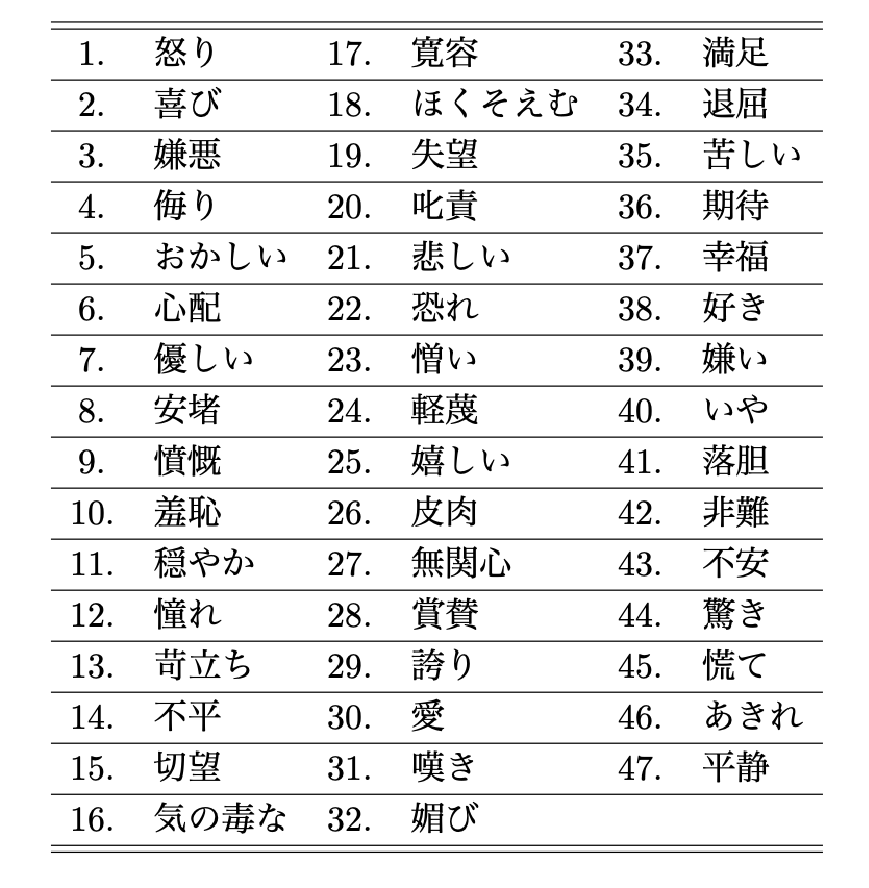
\includegraphics [ width = 1\columnwidth]{Figure/Appendix/6A/Table_Keio-ESD_Emo47.eps}
  \end{minipage}
  
  \end{tabular}
  
  \caption{左:Keio-ESDに収録されている20文節語のモーラ数とアクセント型。アクセントの高低は文字(H:High,L:Low)と◯の高さで示す。
           名詞(11単語)を赤色の行で示す。
           右:発話の際に目標とされた47種類の感情。ともにKeio-ESD付属の説明書より引用。
            }
  \label{fig:Keio-ESD} 

\end{figure}
% ----------------------------------%


%%--------------------------------------------------------------
\section{感情音声の再分類と選別}
\label{sec:Reclass}
%%--------------------------------------------------------------
% ------------------------------
\subsubsection{怒り・悲しみ・喜び実験における感情音声の再分類}
% ------------------------------

\ref{sec:PrepareStimuli}節で述べたように、47種ある感情を話者がどの程度表現できているか、音声を聞いて本当にその感情らしく感じられるかを確かめるために、
実験者3名(著者を含む若年健聴者:日本人大学生と大学院生)で音声の再分類を行った。
手順としては、47感情・11単語の音声を、3人で分担して全て聞き、エクマンの基本6感情(喜び・悲しみ・怒り・恐怖・嫌悪・驚き)\cite{ekman1992argument}に分類した。
実験者はそれぞれ3単語(1名は4単語)$\times$ 47感情分の音声を聞いた。
結果の一部を図\ref{fig:Reclassing6}に示す。
例えば単語「なま」は、「喜び・おかしい・嬉しい・満足・いや」のラベルが付けられた5音声が、実際に聞いてみて「喜び」に感じられた。

% ----------------------------------%
\begin{figure}[h]
  \vspace{50pt}
  \centering
  \includegraphics[width = 1\columnwidth]{Figure/Appendix/6A/Table_Reclassing6.eps}
  \caption{
    単語「なま」「なみ」の分類結果。左から単語、担当した実験者名、基本6感情、該当なし(6感情のどれにも感じられなかった音声)。
    表中の感情語は図\ref{fig:Keio-ESD}右の感情ラベルと一致している。
    }
  \label{fig:Reclassing6}
\end{figure}
% ----------------------------------%


このようにして再分類を行い、「怒り」「悲しみ」「喜び」に分類された音声は合計で176音声であった。


\clearpage
% ------------------------------
\subsubsection{落着き実験における落着き音声の選別}
% ------------------------------
落着き実験では、怒り・悲しみ・喜び実験と同様に実験者3名で分担して全ての感情音声を聞き、「落着き」に感じられる音声を選別した。
その結果の一部を図\ref{fig:ReclassingCal}に示す。
% なお、この段階では判断基準とする感情語を「落着き」ではなく「安心・穏やか」としていた。
% 理由として、ラッセルの感情円環モデル上の快かつ沈静の感情を選ぶ際に、「Calm」「At ease」「Serene」「Relaxed」などがあり、
% それに対応する日本語を「安心・穏やか」としたためである。
選別された音声は合計48音声で、これらについて実際に弁別実験に使用した「怒り」「悲しみ」「喜び」音声との重複はなかった。


% ----------------------------------%
\begin{figure}[h]
  \vspace{10pt}
  \centering
  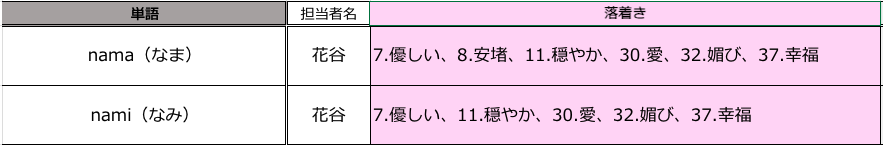
\includegraphics[width = 1\columnwidth]{Figure/Appendix/6A/Table_ReclassingCal.eps}
  \caption{
    単語「なま」「なみ」の選別結果。
    表中の感情語は図\ref{fig:Keio-ESD}右の感情ラベルと一致している。
    }
  \label{fig:ReclassingCal}
\end{figure}
% ----------------------------------%


%%--------------------------------------------------------------
\section{感情音声尺度評定実験}
\label{sec:5Scaling}
%%--------------% ------------------------------
\subsubsection{怒り・悲しみ・喜び実験}
% ----------------------------------------------
抽出された176音声の感情の強さを測定するために、基本6感情について5段階の尺度評定を行った。
また、同時に感情の演技らしさの評価も行なった。
前述の実験者3名全員が参加し、専用のWebページ上で実施した。
暗騒音レベルが約26dBの防音室(YAMAHA, AVITECS)内で行い、機材と提示条件は\ref{sec:ExpCondition}節 "実験機材と提示条件" の内容と同様である。
図\ref{fig:Web_5Scale6}に実際の実験用Webページの一部を示す。

参加者は「再生ボタン」を押し1つの感情音声を聞き、6感情についてそれぞれどの程度感じられたかを、スライダー(図中の丸いボタン)を動かして評定する。
さらに、演技度について「非常に日常的」から「日常会話的」の5段階で評定を行なった。
1つの音声の評価が終わると「次へ」ボタンが表示され、次の音声に移る。
このような手順で、全176音声について評定を行なった。

%%--------------% ------------------------------
\subsubsection{落着き実験}
% ----------------------------------------------
怒り・悲しみ・喜びの弁別実験に用いた30音声(詳細と経緯は\ref{sec:5Scale_Calm}節を参照) + 選別された48の落着き音声に関して、4感情について5段階の尺度評定を行った。
感情の演技らしさの評価も行なった。
実験条件と手順は怒り・悲しみ・喜び実験における尺度評定実験と同じである。
図\ref{fig:Web_5ScaleCal}に実際の実験用Webページの一部を示す。


% ----------------------------------%
\begin{figure}[h]
  \vspace{10pt}
  \centering
  \includegraphics[width = 1\columnwidth]{Figure/Appendix/6A/Web_5Scale6.eps}
  \caption{
    【怒り・悲しみ・喜び実験】感情音声尺度評定の専用Webページのスクリーンショット
    }
  \label{fig:Web_5Scale6}
\end{figure}
% ----------------------------------%

% ----------------------------------%
\begin{figure}[h]
  \vspace{10pt}
  \centering
  \includegraphics[width = 1\columnwidth]{Figure/Appendix/6A/Web_5ScaleCal.eps}
  \caption{
    【落着き実験】感情音声尺度評定の専用Webページのスクリーンショット
    }
  \label{fig:Web_5ScaleCal}
\end{figure}
% ----------------------------------%















%%%%%%%%%%%%%%%%%%%%%%%%%%%%%%%%%%%%%%%%%%%%%%%%%
%% trash
%%%%%%%%%%%%%%%%%%%%%%%%%%%%%%%%%%%%%%%%%%%%%%%%%
% % ----------------------------------%
% \begin{figure}[t]

%   \begin{tabular}{cc}
%   \begin{minipage} {0.5\hsize}
%   \centering
%   \includegraphics [ width = 1\columnwidth]{Figure/Appendix/Web_5Scale6.eps}
%   \end{minipage} & 
  
%   \begin{minipage} {0.5\hsize}
%   \centering
%   \includegraphics [ width = 1\columnwidth]{Figure/Appendix/Web_5ScaleCal.eps}
%   \end{minipage}
  
%   \end{tabular}
  
%   \caption{感情音声尺度評定の専用Webページのスクリーンショット。左:怒り・悲しみ・喜び実験における評定。
%            右:落着き実験における評定。
%             }
%   \label{fig:Web_5Scale} 

% \end{figure}
% % ----------------------------------%




% なお、\ref{sec:morphAngSadHap}で述べたように、実際に弁別実験に用いたのは「おぼろづきよ」を除く10単語である。
